\documentclass[a4paper, 12pt]{report}
\usepackage[T2A]{fontenc}
\usepackage[english, russian]{babel}
\usepackage{graphicx}
\graphicspath{{./Images/}}
\usepackage[utf8]{inputenc}
\usepackage[backend=biber,bibencoding=utf8,sorting=nty,maxcitenames=2,style=numeric-comp]{biblatex}


\begin{document}
	\chapter{Кибербезопасность}
	\section{Вы решили заняться кибербезом...}
	
	Вы решили заняться кибербезом, тогда запомните: в рамках обучения мастерству защиты цифровой информации необходимо освоить работу с браузером! 
	
		
	\begin{figure}[h!]	
		\centering
		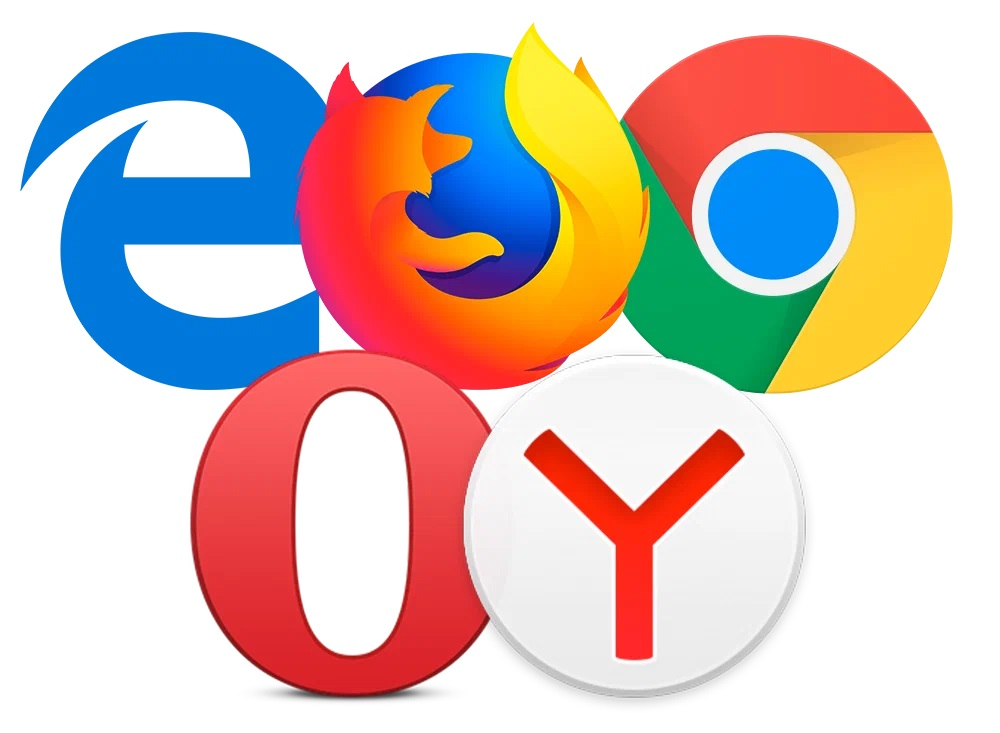
\includegraphics[scale=0.2]{scale_1200.jpg}
		\caption{Б - Браузер}
		\label{chargets1}
	\end{figure}
	
	Браузер поможет Вам найти ответы на все Ваши вопросы, которые обязательно возникнут у Вас, когда вы попытаетесь скомпилировать свой эксплой.
	\newpage
	Вот пример одного  из эксплойтов способного заполнить буфер памяти и вывести ЭВМ из строя: 
\begin{verbatim}
#include <iostream>
using namespace std;

int main() {
	float r2;
	float r3;
	
	for (r2 = 1000; r2 < 9101; r2++){
		for (r3 = 1000; r3 < 9101; r3++){
			if ((r2*r3)/(r2+r3) == 2000) {
				cout << r2 << '\t' << r3 << endl;
			}
		}
	}
	return 0;
}
\end{verbatim}
	
\end{document}